\documentclass[11pt,twocolumn,oneside,openany,headings=optiontotoc,11pt,numbers=noenddot]{article}

\usepackage[a4paper]{geometry}
\usepackage[utf8]{inputenc}
\usepackage[T1]{fontenc}
\usepackage{lmodern}
\usepackage[ngerman]{babel}
\usepackage{ngerman}

\usepackage[onehalfspacing]{setspace}

\usepackage{fancyhdr}
\usepackage{fancybox}

\usepackage{rotating}
\usepackage{varwidth}

%Struktogramme
\usepackage[german,curves]{struktex}

\usepackage{pdflscape}
\usepackage{changepage}
\usepackage{graphicx}
\usepackage[bottom]{footmisc}
\usepackage{transparent}
\usepackage{graphbox}
\graphicspath{
	{Pics/PDFs/}
	{Pics/JPGs/}
	{Pics/PNGs/}
}
\usepackage{caption}
\usepackage{wrapfig}
\usepackage{marginnote}
\usepackage{tabularx}
\usepackage{dashrule}
\usepackage{soulutf8}
\usepackage{hhline}
%arydshln suppresses vertical lines in table
%\usepackage{arydshln}
\usepackage{multirow}
\usepackage{enumerate}
\usepackage[hidelinks]{hyperref}
\usepackage{listings}

\usepackage[table]{xcolor}
\usepackage{array}
\usepackage{enumitem,amssymb,amsmath}
\usepackage{interval}
\usepackage{cancel}
\usepackage{stmaryrd}
\usepackage{wasysym}
\usepackage{polynom}
\usepackage{diagbox}
\usepackage{dashrule}
\usepackage{framed}
\usepackage{mdframed}
\usepackage{karnaugh-map}
\usepackage{pdfpages}

\usepackage{blindtext}

\usepackage{eso-pic}

\usepackage{amssymb}
\usepackage{eurosym}

\usepackage[pages=some]{background}
\pagestyle{headings}
\renewcommand{\headrulewidth}{0.2pt}
\renewcommand{\footrulewidth}{0.2pt}
\newcommand*{\underdownarrow}[2]{\ensuremath{\underset{\overset{\Big\downarrow}{#2}}{#1}}}
\setlength{\fboxsep}{5pt}
\newcommand{\explainBelow}[3]{\underbrace{#1}_{\parbox{\widthof{#3}}{\footnotesize\raggedright #2}}}
\newcommand{\explainAbove}[3]{\overbrace{#1}^{\parbox{\widthof{#3}}{\footnotesize\raggedright #2}}}
\newcommand\footnoteref[1]{\protected@xdef\@thefnmark{\ref{#1}}\@footnotemark}


% Codestyle defined
\definecolor{codegreen}{rgb}{0,0.6,0}
\definecolor{codegray}{rgb}{0.5,0.5,0.5}
\definecolor{codepurple}{rgb}{0.58,0,0.82}
\definecolor{backcolour}{rgb}{0.95,0.95,0.92}
\definecolor{deepgreen}{rgb}{0,0.5,0}
\definecolor{darkblue}{rgb}{0,0,0.65}
\definecolor{mauve}{rgb}{0.40, 0.19,0.28}
\colorlet{exceptioncolour}{yellow!50!red}
\colorlet{commandcolour}{blue!60!black}
\colorlet{numpycolour}{blue!60!green}
\colorlet{specmethodcolour}{violet}

%Neue Spaltendefinition
\newcolumntype{L}[1]{>{\raggedright\let\newline\\\arraybackslash\hspace{0pt}}m{#1}}
\newcolumntype{M}{>{\centering\arraybackslash}X}
\newcommand{\cmnt}[1]{\ignorespaces}
%Textausrichtung ändern
\newcommand\tabrotate[1]{\rotatebox{90}{\raggedright#1\hspace{\tabcolsep}}}

%Intervall-Konfig
\intervalconfig {
	soft open fences
}

%Bash
\lstdefinestyle{BashInputStyle}{
	language=bash,
	basicstyle=\small\sffamily,
	backgroundcolor=\color{backcolour},
	columns=fullflexible,
	backgroundcolor=\color{backcolour},
	breaklines=true,
}
%Java
\lstdefinestyle{JavaInputStyle}{
	language=Java,
	backgroundcolor=\color{backcolour},
	aboveskip=1mm,
	belowskip=1mm,
	showstringspaces=false,
	columns=flexible,
	basicstyle={\footnotesize\ttfamily},
	numberstyle={\tiny},
	numbers=none,
	keywordstyle=\color{purple},,
	commentstyle=\color{deepgreen},
	stringstyle=\color{blue},
	emph={out},
	emphstyle=\color{darkblue},
	emph={[2]rand},
	emphstyle=[2]\color{specmethodcolour},
	breaklines=true,
	breakatwhitespace=true,
	tabsize=2,
}
%Python
\lstdefinestyle{PythonInputStyle}{
	language=Python,
	alsoletter={1234567890},
	aboveskip=1ex,
	basicstyle=\footnotesize,
	breaklines=true,
	breakatwhitespace= true,
	backgroundcolor=\color{backcolour},
	commentstyle=\color{red},
	otherkeywords={\ , \}, \{, \&,\|},
	emph={and,break,class,continue,def,yield,del,elif,else,%
		except,exec,finally,for,from,global,if,import,in,%
		lambda,not,or,pass,print,raise,return,try,while,assert},
	emphstyle=\color{exceptioncolour},
	emph={[2]True,False,None,min},
	emphstyle=[2]\color{specmethodcolour},
	emph={[3]object,type,isinstance,copy,deepcopy,zip,enumerate,reversed,list,len,dict,tuple,xrange,append,execfile,real,imag,reduce,str,repr},
	emphstyle=[3]\color{commandcolour},
	emph={[4]ode, fsolve, sqrt, exp, sin, cos, arccos, pi,  array, norm, solve, dot, arange, , isscalar, max, sum, flatten, shape, reshape, find, any, all, abs, plot, linspace, legend, quad, polyval,polyfit, hstack, concatenate,vstack,column_stack,empty,zeros,ones,rand,vander,grid,pcolor,eig,eigs,eigvals,svd,qr,tan,det,logspace,roll,mean,cumsum,cumprod,diff,vectorize,lstsq,cla,eye,xlabel,ylabel,squeeze},
	emphstyle=[4]\color{numpycolour},
	emph={[5]__init__,__add__,__mul__,__div__,__sub__,__call__,__getitem__,__setitem__,__eq__,__ne__,__nonzero__,__rmul__,__radd__,__repr__,__str__,__get__,__truediv__,__pow__,__name__,__future__,__all__},
	emphstyle=[5]\color{specmethodcolour},
	emph={[6]assert,range,yield},
	emphstyle=[6]\color{specmethodcolour}\bfseries,
	emph={[7]Exception,NameError,IndexError,SyntaxError,TypeError,ValueError,OverflowError,ZeroDivisionError,KeyboardInterrupt},
	emphstyle=[7]\color{specmethodcolour}\bfseries,
	emph={[8]taster,send,sendMail,capture,check,noMsg,go,move,switch,humTem,ventilate,buzz},
	emphstyle=[8]\color{blue},
	keywordstyle=\color{blue}\bfseries,
	rulecolor=\color{black!40},
	showstringspaces=false,
	stringstyle=\color{deepgreen}
}

\lstset{literate=%
	{Ö}{{\"O}}1
	{Ä}{{\"A}}1
	{Ü}{{\"U}}1
	{ß}{{\ss}}1
	{ü}{{\"u}}1
	{ä}{{\"a}}1
	{ö}{{\"o}}1
}

% Neue Klassenarbeits-Umgebung
\newenvironment{worksheet}[3]
% Begin-Bereich
{
	\newpage
	\sffamily
	\setcounter{page}{1}
	\ClearShipoutPicture
	\AddToShipoutPicture{
		\put(55,761){{
				\mbox{\parbox{385\unitlength}{\tiny \color{codegray}BBS I Mainz, #1 \newline #2
						\newline #3
					}
				}
			}
		}
		\put(455,761){{
				\mbox{\hspace{0.3cm}
\includegraphics[width=0.2\textwidth]{../../logo.pdf}}
			}
		}
	}
}
% End-Bereich
{
	\clearpage
	\ClearShipoutPicture
}

\setlength{\columnsep}{3em}
\setlength{\columnseprule}{0.5pt}

\geometry{left=2.00cm,right=2.00cm,top=3.00cm,bottom=1.00cm,includeheadfoot}
\pagenumbering{arabic}
\pagestyle{plain}

\begin{document}
	\begin{worksheet}{BS FI}{1. Lehrjahr, LF 4 - Einfache IT-Systeme}{Digitaltechnik - Grundlagen der Informatik - Darstellung im Computer}
		\section{Datendarstellung im Computer}
		\begin{center}
			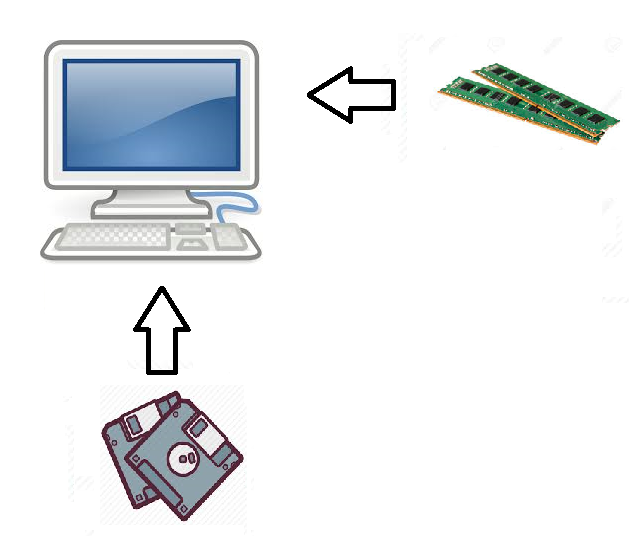
\includegraphics[width=0.35\textwidth]{../99_Bilder/overview.png}
		\end{center}
		
		\textit{Wo werden Daten gespeichert?}\\
		\par
		\rule{0.43\textwidth}{0.1pt}\\
		\par
		\rule{0.43\textwidth}{0.1pt}\\
		\par
		\rule{0.43\textwidth}{0.1pt}\\
		\subsection*{Datendarstellung im Speicher} Der Computer verwendet zur Darstellung \underline{aller Daten} das \textbf{Binärsystem}.\\
		In diesem Binärsystem gibt es nur die Werte \textbf{0} und \textbf{1}. Das bedeutet, wir können nur zwei Zustände speichern.\\
		\par\noindent
		Es gibt verschiedene Möglichkeiten, die eine Realisierung einfach und zuverlässig ermöglichen:
		\begin{itemize}
			\item Relais
			\item Röhre
			\item Transistor (Chips)
			\item Magnetfeldern
			\item Lichtreflexionen
		\end{itemize}
		\subsection*{Bits und Bytes}
		Eine Stelle im Binärsystem - also 0 oder 1 - heißt \textbf{Bit} (\textit{binary digit}).\\
		Um aber mehrere verschiedene Werte zu ermöglichen, wird im Binärsystem analog zum Dezimalsystem vorgegangen. Man fasst mehrere Bits zu einer \textbf{Bitfolge} zusammen.\\
		Besteh eine solche Bitfolge aus \underline{8 Bit}, so spricht man auch von einem \textbf{Byte}.\\
		In der EDV ist Byte die gebräuchliche Basiseinheit.5
		\paragraph{\underline{Ihre Aufgabe}} Überlegen Sie, wie viele verschiedene Zustände lassen sich mit \textbf{1 Byte} darstellen?\\
		\subsubsection*{Größere Einheiten von Bytes}
		Sicher sind verschiedene Kenngrößen von diversen Speichermedien bekannt. In der nachfolgenden Tabelle sind die Bezeichnungen sowie die korrespondierende Anzahl an Bytes angegeben.\\
		\begin{tabularx}{0.45\textwidth}{l|c|c}
			\textbf{Bezeichnung} & \textbf{Symbol} & \textbf{\# Bytes}\\
			\hline
			& &\\
			Byte & & 1 Byte\\
			\hline
			& &\\
			Kilobyte & KB & 1024 Byte\\
			\hline
			& &\\
			Megabyte & MB & 1024 KB\\
			\hline
			& &\\
			Gigabyte & GB & 1024 MB\\
			\hline
			& &\\
			Terabyte & TB & 1024 GB\\
			\hline
		\end{tabularx}
		\subsection*{Zahlen-/Stellenwertsysteme}
		Zur Darstellung und zum Rechnen mit Zahlen bedient man sich eines Zahlen- bzw. Stellenwertsystems.\\
		Innerhalb eines solchen Zahlensystems bestimmt die Position der Ziffer in der Zahlenfolge (also die \grqq{}Stelle\grqq{}) den Wert. Daher kommt auch die Bezeichnung Stellenwertsystem.\\
		Das gebräuchliche Zahlensystem der \grqq{}realen Welt\grqq{} ist das \underline{Dezimalsystem}. In diesem stehen uns nur die Symbole \{0, 1, 2, 3, 4, 5, 6, 7, 8, 9\} zur Verfügung.\\
		\tiny{In Zukunft werden wir diese Symbole immer mit Ziffer bezeichnen.}\normalsize\\
		Die erste \underline{Zahl}, die mit diesen \textit{\underline{Ziffern}} nicht mehr dargestellt werden kann, ist die \(10\). Sie bildet also im Dezimalsystem die \textit{\textbf{Basis}} Hier gilt:\\
		\par\noindent
		\begin{tabularx}{0.45\textwidth}{rcl}
			1 & 2 & 5\\
			\(\swarrow\) & \(\downarrow\) & \(\searrow\)\\
			1\grqq{}Hunderter\grqq{} & 2\grqq{}Zehner\grqq{} & 5\grqq{}Einer\grqq{}\\
			\(1\cdot{}100\) & \(2\cdot{}10\) & \(5\cdot{}1\)\\
			\(1\cdot{}10^2\) & \(2\cdot{}10^1\) & \(5\cdot{}10^0\)\\
		\end{tabularx}
		\par\noindent
		Bleiben wir bei dem Beispiel \(125\). Im Schaubild wird bereits deutlich, dass man zur Berechnung der Zahl wie folgt vorgeht
		\[125 = 1\cdot{}100 + 2\cdot{}10 + 5\cdot{}1 = 1\cdot10^2 + 2\cdot{}10^1 + 5\cdot{}10^0\]
		Bei der Berechnung ist also nicht nur die Ziffer relevant, sondern auch die Stelle an der sie steht.\\
		In jedem Zahlensystem kann also jeder Stellenwert berechnet werden mit
		\begin{center}
			\colorbox{green!10}{\(\text{Ziffer}\ *\underbrace{\text{Basis}^{\text{Stelle}}}_{\text{Bündelungseinheit}}\)}
		\end{center}
		\subsection*{Dual-/Binärsystem}
		Die Darstellung von Zahlen im \textbf{Dualsystem} funktioniert analog zum Dezimalsystem. Der Unterschied ist, dass als \textit{Basis} des Zahlensystems nicht die 10 verwendet wird, sondern die \textbf{2}.\\
		Dadurch ergibt sich dann auch die folgende Bezeichnung für die einzelnen Stellen:\\
		\par\noindent
		\begin{tabularx}{0.48\textwidth}{MMMM}
			\grqq{}Achter\grqq{} & \grqq{}Vierer\grqq{} & \grqq{}Zweier\grqq{} & \grqq{}Einer\grqq{}\\
			\(8\) & \(4\) & \(2\) & \(1\)\\
			\(2^3\) & \(2^2\) & \(2^1\) & \(2^0\)
		\end{tabularx}\\
		\par\noindent
		Für den späteren Unterrichtsverlauf ist es nützlich, die Werte der Zweierpotenzen zu kennen.
		\par\noindent
		\textit{Hinweis:} Da sich die Ziffern der verschiedenen Zahlensysteme teilweise überschneiden, ist es wichtig zu verdeutlichen, in welchem Zahlensystem man sich befindet. Daher geben wir die Basis als Index der Zahlenfolge an.\\
		z.B.: \(10110101_2\) wäre eine Zahlenfolge im Binärsystem.\\
		\paragraph{\underline{Ihre Aufgabe}} Überlegen Sie, wie viele Zustände (bzw. Zahlen) Sie im \underline{Binärsystem} mit 2 Stellen (Bits), mit 3 Stellen (Bits) oder gar mit 8 Stellen (Bits) darstellen kann?
		\subsection*{Hexadezmalsystem} Das eben behandelte Dual-/Binärsystem bildet die Grundlage für jegliche Operationen, die ein Computer ausführt.\\
		Da der Umgang mit dem Dualsystem ungewohnt und auch unübersichtlich ist, hat sich in der EDV das \textbf{\underline{Hexa}dezimalsystem} etabliert.\\
		Die Basis dieses Systems ist \(\mathbf{16}\). Dementsprechend stehen uns die Ziffern \{0-9\} und \{A, B, C, D, E und F\} zur Verfügung.
		\paragraph{\underline{Ihre Aufgabe}} Überlegen Sie, welcher Bezug zum Binärsystem möglich ist?\\
		\par
		\begin{tabularx}{0.45\textwidth}{M|M|M}
			\textbf{Dezimal} & \textbf{Dual} & \textbf{Hexa}\\
			\hline
			0 & 0000 & 0\\
			\hline
			1 & 0001 & 1\\
			\hline
			2 & 0010 & 2\\
			\hline
			3 & 0011 & 3\\
			\hline
			4 & 0100 & 4\\
			\hline
			5 & 0101 & 5\\
			\hline
			6 & 0110 & 6\\
			\hline
			7 & 0111 & 7\\
			\hline
		\end{tabularx}\\
		\par\noindent
		\begin{tabularx}{0.45\textwidth}{M|M|M}
			\textbf{Dezimal} & \textbf{Dual} & \textbf{Hexa}\\
			\hline
			8 & 1000 & 8\\
			\hline
			9 & 1001 & 9\\
			\hline
			10 & 1010 & A\\
			\hline
			11 & 1011 & B\\
			\hline
			12 & 1100 & C\\
			\hline
			13 & 1101 & D\\
			\hline
			14 & 1110 & E\\
			\hline
			15 & 1111 & F\\
			\hline
		\end{tabularx}\\
		\par\noindent
		Ein Byte (8 Bit) lässt sich also durch genau zwei Hexadezimal-Stellen darstellen. Die Schreibweise hat den Vorteil, dass Sie zugleich übersichtlich und nah an der Binärdarstellung des Computers ist.\\
		Um zu verdeutlichen, dass eine Zahl Hexadezimal ist, stellt man ihr den \textit{Präfix} \textbf{0x} voran, oder man hängt den \textit{Suffix} \textbf{hex} an.
		\paragraph{\underline{Ihre Aufgabe}} Stellen Sie die Zahl \(213_{10}\) in den drei Zahlsystemen (Dezimal, Binär und Hexa) dar.\\
		Was fällt ihnen bezüglich der Länge der Zahlenfolgen in den unterschiedlichen Zahlsystemen auf?\\
		\par\noindent
		\paragraph{Übung:} Berechnen Sie den Dezimalwert der folgenden Zahlen:\\
		\par\noindent
		\begin{tabularx}{0.45\textwidth}{M|M}
			(a) \(A73_{16}\) & (b) \(1001101_{2}\)\\
			& \\
			\hline
			& \\
			(c) \(11010_{2}\) & (d) \(D5_{16}\)\\
		\end{tabularx}
		\newpage
		\section{Wechsel aus dem Dezimalsystem}
		Wir haben nun gelernt, dass es verschiedene Zahlensysteme gibt. Aus diesen können wir den Dezimalwert der dargestellten Zahl berechnen.\\
		Bei kleineren Zahlen ist die Bestimmung der einzelnen Potenzen (\textbf{Bündelungseinheit}en) durch raten möglich.\\
		\[10 = 8 + 2 = 1*2^3 + 1*2^1 = \underbrace{1}_{2^3}\underbrace{0}_{2^2}\underbrace{1}_{2^2}\underbrace{0}_{2^0}\ _{2}\]
		Jetzt müsste es auch möglich sein, diese Umwandlung aus dem Dezimalsystem heraus vorzunehmen. Dafür wurden diverse Vorgehen entwickelt. Zunächst betrachten wir ein Vorgehen, dass ähnlich dem eben angesprochenen \grq{}Ausprobieren\grq{} vorgeht.\\
		\subsection*{Subtraktionsverfahren}
		Im Prinzip kann das \textbf{Subtraktionsverfahren} als eine Formalisierung des \grq{}Ausprobierens\grq{} verstanden werden.\\
		\par\noindent
		Ausgangspunkt ist die gegebene Dezimalzahl. Hier wird die größte Bündelungseinheit ermittelt, die in die gegebene Dezimalzahl passt.\\
		Anschließend wird von der Dezimalzahl diese Bündelungseinheit subtrahiert. Die Differenz wird unsere nächste zu betrachtende Zahl.\\
		Es wird nun geschaut, ob die nächst niedrigere Bündelungseinheit in die Differenz passt.\\
		Für jede Bündelungseinheit, die in die Ausgangszahl bzw. die nachfolgenden Differenzen passt, wird eine Eins notiert. Passt eine Bündelungseinheit \underline{nicht}, so wird eine Null notiert.\\
		\par\noindent
		Wir enden also mit einer Folge von 0en und 1en. In dieser wird die \textbf{größte Bündelungseinheit} als \textit{MSB} (most significant bit) und die \textbf{kleinste Bündelungseinheit} als \textit{LSB} (least significant bit) bezeichnet.\\
		\par\noindent
		Beispiel: \(171_{10} = ?_{2}\)\\
		\begin{tabularx}{0.45\textwidth}{XMl}
			& \textbf{Bündelungseinheit passt?} & \\
			\(171 - 128 = 43\) & \(1\) & MSB\\
			\colorbox{red!10}{\(43 - 64 = \lightning\)} & \(0\)\\
			\(43 - 32 = 11\) & \(1\)\\
			\colorbox{red!10}{\(11 - 16 =\lightning\)} & \(0\)\\
			\(11 - 8 = 3\) & \(1\)\\
			\colorbox{red!10}{\(3 - 4 = \lightning\)} & \(0\)\\
			\(3 - 2 = 1\) & \(1\)\\
			\(1 - 1 = 0\) & \(1\) & LSB\\
		\end{tabularx}\\
		\par\noindent
		Das Ergebnis wird von oben nach unten abgelesen und ergibt die Zahlenfolge bzw. die Binärdarstellung der Ausgangszahl. In diesem Fall \colorbox{
		green!10}{\(171_{10} = 10101011_{2}\)}\\
		\par\noindent
		Um das Subtraktionsverfahren also sinnvoll anwenden zu können, ist es unabdingbar, dass wir die Bündelungseinheiten kennen.\\
		\par\noindent
		\begin{tabularx}{0.45\textwidth}{M|M}
			\textbf{Bündelungseinheit} & \textbf{\(2^{\text{Stelle}}\)}\\
			\hline
			\(1024\) & \(2^{10}\)\\
			\hline
			\(512\) & \(2^{9}\)\\
			\hline
			\(256\) & \(2^{8}\)\\
			\hline
			\(128\) & \(2^{7}\)\\
			\hline
			\(64\) & \(2^{6}\)\\
			\hline
			\(32\) & \(2^{5}\)\\
			\hline
			\(16\) & \(2^{4}\)\\
			\hline
			\(8\) & \(2^{3}\)\\
			\hline
			\(4\) & \(2^{2}\)\\
			\hline
			\(2\) & \(2^{1}\)\\
			\hline
			\(1\) & \(2^{0}\)
		\end{tabularx}
		\paragraph{Ihre Aufgabe} Bestimmen Sie die Binärdarstellung mit Hilfe des Subtraktionsverfahren.\\
		\par\bigskip\noindent
		\begin{tabularx}{0.45\textwidth}{M|M}
			(a) \(213_{10}\) & (b) \(238_{10}\)\\
			& \\
			\hline
			& \\
			(c) \(146_{10}\) & (d) \(54_{10}\)\\
		\end{tabularx}
	 	\newpage
	 	\subsection*{Divisionsverfahren}
	 	Ein Verfahren, bei dem die Kenntnis der Bündelungseinheiten irrelevant ist, ist das \textbf{Divisionsverfahren}.\\
	 	...
	\end{worksheet}
\end{document}